\documentclass[a4paper,notumble]{leaflet}
\usepackage{graphics,titlesec}
	\graphicspath{{./Figures/}}
\usepackage[dutch]{babel}
\usepackage{multirow,multicol,array}
\usepackage{framed,libertine-otf,fontawesome}
\usepackage{microtype}
\usepackage[dvipsnames,usenames,svgnames]{xcolor}
\usepackage{hyperref}
\usepackage{flowfram}
\usepackage{caption}
\usepackage{tikz}
%\usepackage{amsmath,amssymb}
\usepackage{transparent}
\definecolor{breastpink}{RGB}{234,128,176}
% Make a border along the top of each page
\setmargins{15mm}{15mm}{7mm}{7mm}
\vtwotonetop{1cm}{0.6\paperwidth}{[RGB]{234,128,176}}{topleft}{0.4\paperwidth}{[RGB]{234,128,176}}{topright}
\vtwotonebottom[1,6]{1cm}{0.6\paperwidth}{[RGB]{234,128,176}}{bottomleft}{0.4\paperwidth}{[RGB]{234,128,176}}{bottomright}

\titleformat*{\section}{\bf\color{purple!80!red}\sffamily}
\titleformat*{\subsection}{\small\bf\color{purple!80!red}\sffamily}
%\title{\huge\color{breastpink}Bevolkingsonderzoek borstkanker}
%\author{}
%\date{}
%\subtitle{\color{breastpink}Uitnodiging}
%\pagestyle{empty}
%\AddToBackground{1}{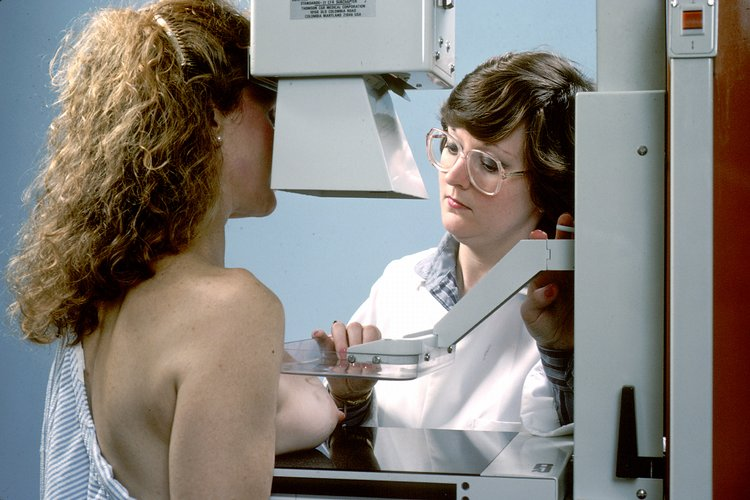
\includegraphics[width=\textwidth]{mammogram_proced.jpg}}
%\AddToBackground{4}{\includegraphics[width=\textwidth]{testeigenschappendiagram.pdf}}
%\AddToBackground{6}{\includegraphics[width=\textwidth]{./Figures/semper_invicta.pdf}}
\hbadness=2000 % geeft mate van stretching weer van boxes, hoe hoger de waarde des te kleiner kans dat je waarschuwing underfull of overfull box krijgt.
%\renewcommand{\labelitemi}{\scriptsize$\blacksquare$}
\begin{document}
\begin{titlepage}
	\title{%
		\bf\sffamily\huge\color{purple!80!red}Bevolkingsonderzoek borstkanker
	}
	\author{%
		\sffamily Uitnodiging
	}
	\date{}
\end{titlepage}
\maketitle
%%%%%%%%%%%%%%%%%%%%%%%%%%%%%%%%%%%%%%%%%%%%%%%%%%%%%%%%%%%%%%%%%%%%%%%%%%%%%
\section{Wat is een bevolkingsonderzoek voor borstkanker?}
Vanaf uw 50ste tot uw 75ste levensjaar ontvangt u en alle andere vrouwen van deze leeftijden tweejaarlijks een uitnodiging om een röntgenfoto van uw borsten te laten maken. Een dergelijke foto wordt een mammogram genoemd. Uw borsten worden hierbij tussen twee platen vastgezet. Verscheidene artsen bepalen met de mammogram of er abnormaliteiten in uw borst bevinden. Als de arts een voorloper van borstkanker in de mammogram ziet, dan moet dit worden bevestigd door een biopt te nemen. Bij het nemen van een biopt wordt het afwijkend weefsel van uw borsten weggenomen. De uitslag van de mammogram garandeert dus niet of u wel of niet kanker hebt.
\vfil
\begin{center}
	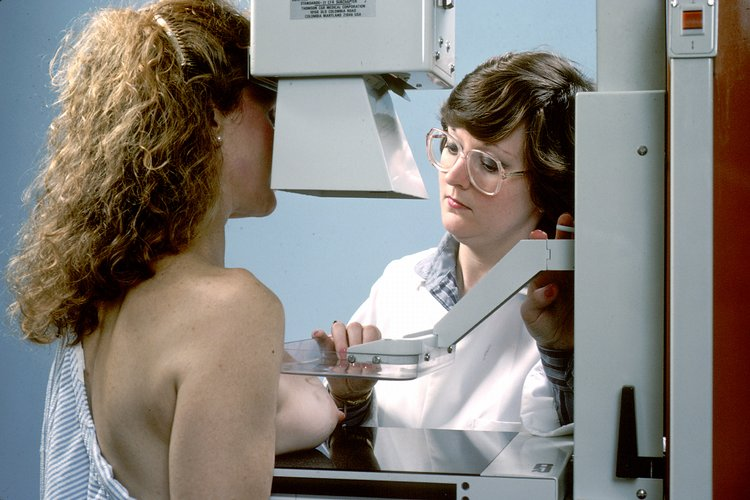
\includegraphics[width=\textwidth]{mammogram_proced.jpg}
\end{center}
\newpage
%%%%%%%%%%%%%%%%%%%%%%%%%%%%%%%%%%%%%%%%%%%%%%%%%%%%%%%%%%%%%%%%%%%%%%%%%%%%%
\section{Wat is borstkanker?}
Borstkanker is een kwaadaardig gezwel in de borst. De kankercellen kunnen het gezonde borstweefsel verdringen, als ze niet worden verwijderd of wegbestraald. Ook kunnen de kankercellen zich verspreiden naar andere delen van het lichaam.
\section{Is deelname aan het bevolkingsonderzoek verplicht?}
Deelname aan het onderzoek is vrijwillig. In deze folder worden alle voor- en nadelen en hun gewichten besproken.
\section{Wat zijn de kosten van deelname aan het onderzoek?}
Het maken van de mammogram is gratis. Het nemen van een biopt in ziekenhuis behoort niet tot het bevolkingsonderzoek. De vergoeding van deze kosten hangt af van uw verzekeringspakket bij uw zorgverzekeraar. Informeer uw zorgverzekeraar naar de mate van vergoeding van deze kosten.
%%%%%%%%%%%%%%%%%%%%%%%%%%%%%%%%%%%%%%%%%%%%%%%%%%%%%%%%%%%%%%%%%%%%%%%%%%%%%
\section{Wat is het nut van het bevolkingsonderzoek?}
Deelnemen aan het bevolkingsonderzoek voor borstkanker heeft zijn voor- en nadelen.
\subsection{Overlevingskans \& kans op borstkanker}
Vanaf het vijftigste levensjaar is de kans om borstkanker te krijgen zeer verhoogd. Daarom omvat de totale aantal borstkankerpatiënten een groot aandeel van vrouwen in de vijftig. 1~\% van vrouwen in de vijftig heeft borstkanker. Dit komt neer op ongeveer 20.000 vrouwen met borstkanker.\par
Bij de invoering van het bevolkingsonderzoek in 1990 zorgde het vroeg opsporen van nog geen klachtengevende borstkanker langere levensverwachtiging. Nu is echter de behandeling van borstkanker zo goed dat het bevolkingsonderzoek bijna geen verlaging in het aantal sterftegevallen door borstkanker geeft. Van de 1 miljoen vrouwen die tweejaarlijks aan het bevolkingsonderzoek deelnemen, sterven 1000 minder vrouwen aan borstkanker. Deelname aan het bevolkingsonderzoek vermindert sterfte aan borstkanker met 25 \% in vergelijking tot geen deelname.
\subsection{Wat zijn de uitslagen van mammogram en hun betekenis?}
De mammogram is niet onfeilbaar in het bevestigen of iemand kanker in vroegstadium heeft of niet. 3 op 10 vrouwen met een borstkankergezwel worden verteld geen borstkanker te hebben. Een borstkankergezwel zal in de volgende uitnodiging worden gedetecteerd of de vrouwen vertonen binnen 2 jaar klachten. De mammogram verklaart ook gezonde vrouwen een voorloper van kanker te hebben. 2 op 100 gezonde vrouwen krijgen onterecht deze uitslag. Deze vrouwen worden verwezen naar het ziekenhuis voor het nemen van een biopt. Deze uitslag en verwijzing is zowel geestelijk als lichamelijk belastend.\par
Nog een nadeel van het vroeg opsporen van een kankergezwel is overbehandeling. Als zowel de mammogram als het biopt bevestigen dat een borstkankergezwel aanwezig is, dan wordt een (gedeeltelijk) borstverwijdering uitgevoerd. In dit vroege stadium kunnen de artsen niet voorspellen hoe agressief het borstkankergezwel is. Sommige borstkankergezwellen groeien snel en zaaien uit, terwijl andere langzaam groeien en nooit klachten zullen geven. Voor vrouwen met de laatstgenoemde borstkankergezwellen zullen dus onnodig borstamputaties ondergaan. Dit wordt overbehandeling genoemd. 30~\% van vrouwen met een vroeg opgespoorde borstkankergezwel lijden aan overbehandeling(OB).
\newpage
\includegraphics[width=\textwidth]{testeigenschappendiagram.pdf}
\captionof*{figure}{%
In een groep van vrouwen in de vijftig heeft een klein deel een nog niet klachtengevende borstkankergezwel en een groot deel gezonde borsten. Van de vrouwen met een borstkankergezwel worden $\frac{3}{10}$ gemist. Zij worden verklaard geen kanker (GK) te hebben. Een gedeelte van vrouwen met een gedecteerde borstkankergezwel zal nooit klachten van het gezwel krijgen en sterven aan borstkanker. Dit deel wordt overbehandeld(OB). Ten slotte is er een kleine groep van gezonde vrouwen met geen borstkankergezwel op basis van mammogram toch verklaard worden kanker (K) te hebben. Deze groep krijgt na het nemen van biopt in het ziekenhuis te horen dat het fout nieuws is.
}
\newpage
%\begin{center}
%	\includegraphics[width=\textwidth]{testeigenschappendiagram.pdf}
%\end{center}
%\begin{center}
%	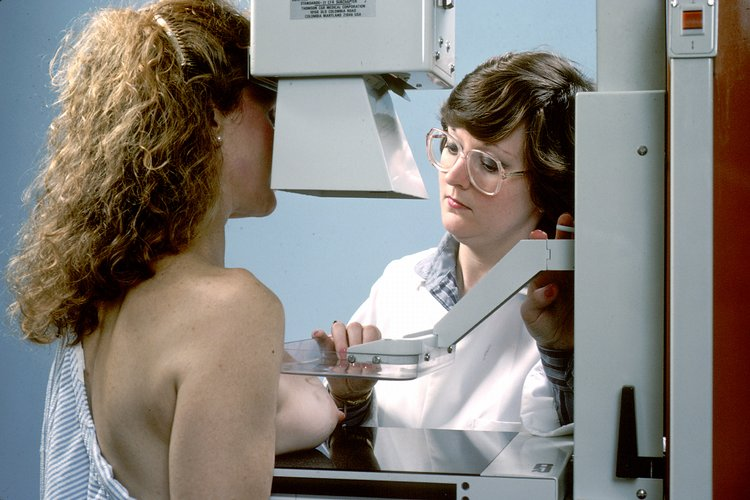
\includegraphics[scale=1]{mammogram_proced.jpg}
%\end{center}

%Hierdoor detecteren de artsen borstkanker, voordat u klachten van borstkanker ervaart.

\section{Waar moet ik opletten na een niet-afwijkende mammogram?}
Een niet-afwijkende mammogram betekent niet dat u geen kankergezwel hebt. In de volgende gevallen bezoek uw huisarts zo spoedig mogelijk:
\begin{itemize}
	\item als u een knobbel in uw borst voel
	\item als er kuiltjes in de huid zijn
	\item als er een plaatselijke verdikking is van de huid
	\item als bloed uit uw tepel komt
	\item als uw tepel verandert
	\item als uw borst anders voelt.
\end{itemize}

\section{Contactgegevens}
\begin{tabular}{cl}
	\multicolumn{2}{l}{\bf Ministerie van Zorg en Welzijn}\\
	\faEnvelope & \href{mailto:e.namani@student.rug.nl}{e.namani@student.rug.nl}\\
	\faPhone & +31 6 28 21 49 68\\
	\faMapMarker & P.O. Box 1 | 3720 BA Bilthoven \\
	\\
	\faChain & \url{https://www.rivm.nl/Onderwerpen}\\
	\faFacebookOfficial & \url{https://www.facebook.com/RIVMnl}\\
	\faTwitter & \url{https://twitter.com/rivm}\\
\end{tabular}
\newpage
\phantom{hoi}
\vfill
\begin{center}
	\includegraphics[scale=.25]{./Figures/semper_invicta.pdf}\\[\baselineskip]
\footnotesize{
		\textcopyright\ 2018 Edon Productions |
		    	vervaardigd met \LaTeXe
			        }
\end{center}
\end{document}
